\documentclass[]{IEEEtran}

% Your packages go here
\usepackage[utf8]{inputenc}
\usepackage{graphicx}
\usepackage{float}
\usepackage{listings}
\usepackage{xcolor}
%listings settings
\definecolor{codegreen}{rgb}{0,0.6,0}
\definecolor{codegray}{rgb}{0.5,0.5,0.5}
\definecolor{codepurple}{rgb}{0.58,0,0.82}
\definecolor{backcolour}{rgb}{0.95,0.95,0.92}
\definecolor{codeblue}{rgb}{0,0.8,0.99}
\definecolor{codeyellow}{rgb}{0.6,0.5,0}


\lstdefinestyle{vim_like}{
  backgroundcolor=\color{backcolour},   
  commentstyle=\color{codegreen},
  keywordstyle=\color{codeyellow},
  numberstyle=\tiny\color{codegray},
  stringstyle=\color{codepurple},
  basicstyle=\ttfamily\footnotesize,
  breakatwhitespace=false,         
  breaklines=true,                 
  captionpos=b,                    
  keepspaces=true,                 
  numbers=left,                    
  numbersep=5pt,                  
  showspaces=false,                
  showstringspaces=false,
  showtabs=false,                  
  tabsize=2
}
\lstset{style=vim_like}

\markboth{MO443 Digital Image Processing}{}

\begin{document}
  \title{Project 5 - Image Compression}
  \author{Thales Mateus Rodrigues Oliveira (RA 148051)
    \thanks{ra148051@students.ic.unicamp.br}
  }
  \maketitle
  
  \begin{abstract}
    In this project, it was given the task of implementing an image compression algorithm, using mathematical formulations. To fulfill the requirements, the solution uses the Principal Component Analysis (PCA) approach. It was able to generate the compressed images for some cases, with some degree of information loss. The details of the implementation are explained in this report.
  \end{abstract}
  
\section{Introduction}

Principal Component Analysis (PCA) is a technique used for reducing the dimensionality of data, by applying Single Value Decomposition (SVD) to the image matrix, and selecting a reduced number of axis components. In this work, the implementation of the technique was done, and tests performed, changing the number of selected components and evaluating by quantitative indicators. The next sections explains the implemented algorithm, the experiments realized and the output analysis.
\\
The code, along with the input files is delivered in the compressed file THALES\_MATEUS\_RODRIGUES\_OLIVEIRA\_148051.zip, in the Google Classroom. The report is sent via e-mail.
\section{The Program}
 
The program was implemented with Python 3.7.3. The libraries used and their respective versions are OpenCV 4.1.0 and Numpy 1.16.4.

\subsection{How to execute it}

The project has a Makefile available to help performing some actions on it. The Makefile has 3 basic instructions: clean, build and exec. Clean instruction removes generated images stored in the \textbf{output} folder, the execution code in \textbf{bin} folder and the folders itself. The Build instruction creates the \textbf{output} and \textbf{bin} folders, and moves the source code to \textbf{bin}. The Exec instruction executes the code with images in the \textbf{input} folder. Listing \ref{code:makefile} provides examples of how to execute the three instructions in a terminal.
\begin{lstlisting}[language=sh, caption={Makefile usage example}, label={code:makefile}]
  #clean environment, deletes output and bin folders and their content
  make clean
  
  #prepare the environment for code execution
  make build 

  #executes code
  make exec
\end{lstlisting}

\subsection{Input}

The program does not have an input argument by default, the input images are listed in code, and they are expected to be stored in the \textbf{input} folder. Listing \ref{code:input} shows how images are listed to be executed in code. The $images$ tuple is implemented in $src/main.py$.

\begin{lstlisting}[language=Python, caption={Input images inside code}, label={code:input}]
  # for inserting other images, add tem to /input folder and list them here
  images = (
      'baboon',
      'monalisa',
      'peppers',
      'watch'
  )
\end{lstlisting}

\subsection{Output}
The output of the program is a series of compressed images based on the input ones, changing the number of selected components from the SVD. The output images are stored in the \textbf{output} folder, and they are labeled by concatenating the image name and the number of selected components (\textit{e.g.: baboon\_10.png})

\subsection{Implementation}
The function which implements the compression operation is defined in the \textit{src/compress.py} file, and it is named \textit{apply\_svd()}. As explained in the project description\cite{PROJECT:5}, as the result of the SVD gives the matrix of eigenvalues in the decreasing order, the first elements of the eigenvalues and eigenvectors matrices contributes more to the final result of the image (has higher contribution in the image formation). Therefore, keeping only few of these elements may result in images with lower quality, which requires less capacity of storage. The function receives the original image, and the number of components to be kept. Listing \ref{code:svd} shows keyparts of implementation. It was inspired by Algorithm I from the project description. As we can see, it applies the SVD for every single color channel, selects the desired number of components from each matrix, and then builds the image back.

\begin{lstlisting}[language=Python, caption={Implementation of Compression with PCA}, label={code:svd}]
def apply_svd(img, n_components):
  """
  It applies image compression method using SVD decomposition.  

  Keyword arguments:
  img -- the image to be compressed
  n_components -- the number of svd components to be considered
  """

  # initialize result array
  result = np.zeros_like(img.astype(np.double))

  # do the SVD for every color channel separately
  w_b, u_b, vt_b = np.linalg.svd(img[:, :, 0].astype(np.double))
  w_g, u_g, vt_g = np.linalg.svd(img[:, :, 1].astype(np.double))
  w_r, u_r, vt_r = np.linalg.svd(img[:, :, 2].astype(np.double))

  # transforms U to matrix form
  u_b = np.diag(u_b)
  u_g = np.diag(u_g)
  u_r = np.diag(u_r)

  # separates the desired number of components
  w_result_b = w_b[:, 0:n_components]
  w_result_g = w_g[:, 0:n_components]
  w_result_r = w_r[:, 0:n_components]
  u_result_b = u_b[0:n_components, 0:n_components]
  u_result_g = u_g[0:n_components, 0:n_components]
  u_result_r = u_r[0:n_components, 0:n_components]
  vt_result_b = vt_b[0:n_components, :]
  vt_result_g = vt_g[0:n_components, :]
  vt_result_r = vt_r[0:n_components, :]

  # builds the compressed image by multiplying the desired components
  result[:, :, 0] = w_result_b.dot(u_result_b.dot(vt_result_b))
  result[:, :, 1] = w_result_g.dot(u_result_g.dot(vt_result_g))
  result[:, :, 2] = w_result_r.dot(u_result_r.dot(vt_result_r))

  return result

\end{lstlisting}

\subsubsection{Evaluating the Compression}
With the objective of evaluating the compression, two quantitative indicators were implemented: the compression rate, and the root mean-squared error. The formulations of both indicators are given in the project description\cite{PROJECT:5}. Listing \ref{code:eval} shows the implementation. After calculating the values, their are printed in the standard output.

\begin{lstlisting}[language=Python, caption={Evaluation of Compressed Images}, label={code:eval}]
def evaluate_compression(original, compressed, name, n_components):
  """
  It quantitatively evaluates a compression, by calculating the compression rate and the Root Mean-Squared Error (RMSE)

  Keyword arguments:
  original -- the original image (numpy array)
  compressed -- the compressed image (numpy array)
  name -- the image name
  n_components -- the number of components considered for the compression
  """
  original_size = os.path.getsize('input/' + name + '.png')
  compressed_size = os.path.getsize('output/' + name + '_' + str(n_components) + '.png')
  # calculates the compression rate by dividing the storage sizes
  compression_rate = compressed_size/original_size
  # Calculates RMSE
  rmse = math.sqrt((((original - compressed)**2).sum())/(original.shape[0]*original.shape[1])) 
  print("\t\t" + "Compression rate: " + str(compression_rate) + " RMSE:" + str(rmse))
  
  \end{lstlisting}

\section{Experiments}
The \textit{src/main.py} file executes the test pipeline. The idea is the following: for each input image, for number of components, generate the compressed versions and evaluate the result. The input images are stored in \textbf{input} folder as mentioned before, and their names and dimensions are listed in table \ref{table:input}. The input images are shown in figure \ref{fig:input-images}

\begin{table}[h!]
\centering
\begin{center}
\begin{tabular}{ |c|c| } 
 \hline
 Image Names & Dimensions (width x height) \\
 \hline
  baboon.png &  512 x 512\\ 
 \hline
  monalisa.png & 256 x 256\\
 \hline
  peppers.png &  512 x 512\\ 
 \hline
  watch.png & 1024 x 768\\
 \hline
\end{tabular}
\caption{Input images used in experiments}
\label{table:input}
\end{center}
\end{table}

\begin{figure}[H]
  \centering
  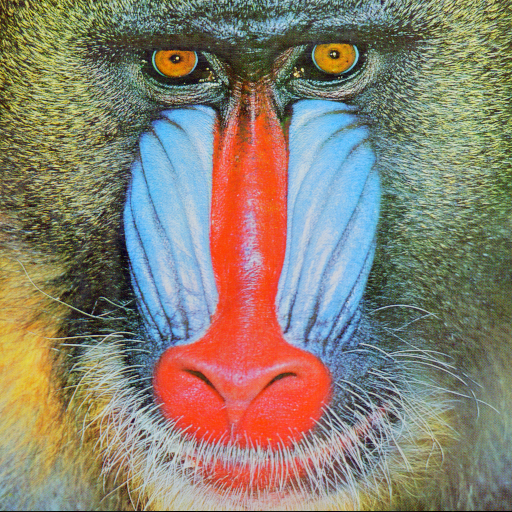
\includegraphics[width=0.4\hsize]{../input/baboon.png}
  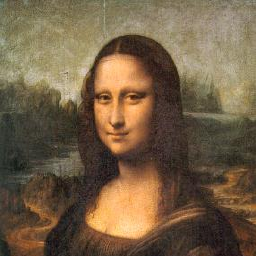
\includegraphics[width=0.4\hsize]{../input/monalisa.png}
  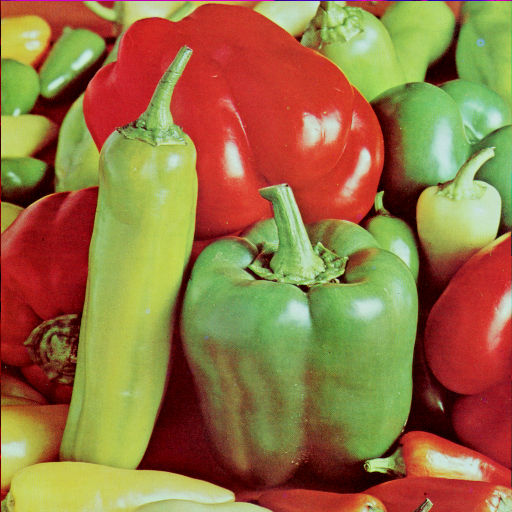
\includegraphics[width=0.4\hsize]{../input/peppers.png}
  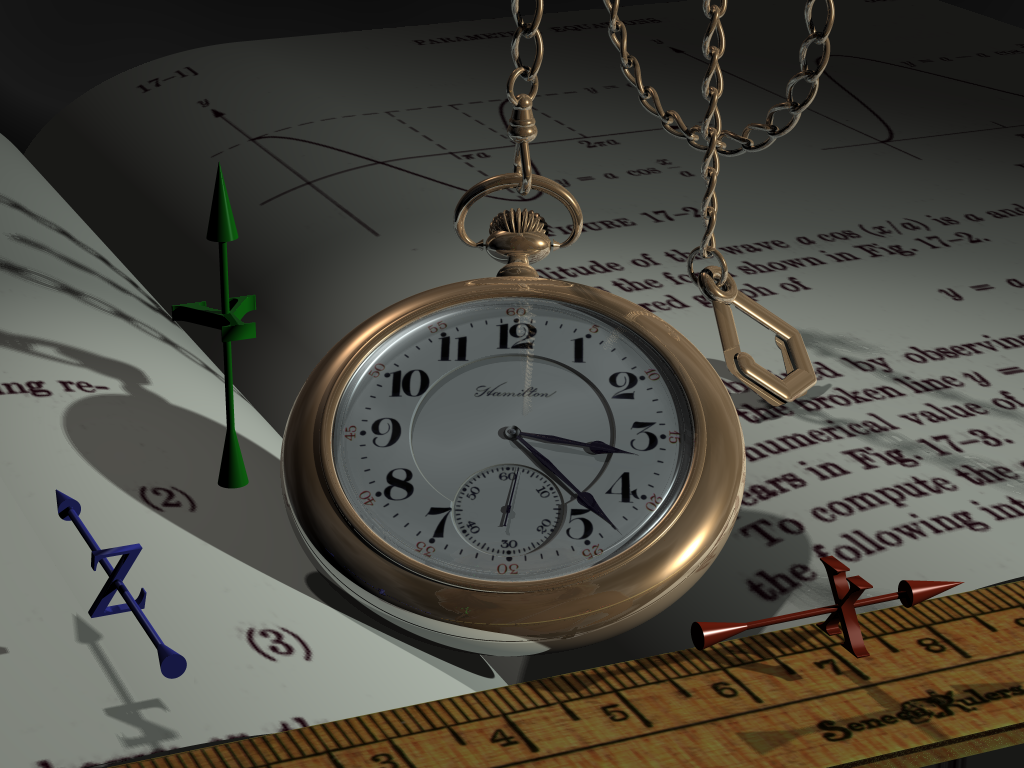
\includegraphics[width=0.4\hsize]{../input/watch.png}
  \caption{Input images used in experiments. a) Baboon. b) Monalisa c) Peppers d) Watch}
  \label{fig:input-images}
\end{figure}

The number of components used were taken from the example given by the project description\cite{PROJECT:5}. Table \ref{table:components} lists the used values.

\begin{table}[h!]
  \centering
  \begin{center}
  \begin{tabular}{ |c| } 
   \hline
   Number of components used in tests \\
   \hline
    1\\ 
   \hline
    5\\
   \hline
    10\\ 
   \hline
    20\\
   \hline
    30\\
   \hline
    40 \\ 
   \hline
   50 \\
   \hline
  \end{tabular}
  \caption{Number of components used in tests}
  \label{table:components}
  \end{center}
  \end{table}

As we have 4 input images and 7 different component values, we have 28 images of output. The output images are stored in the \textbf{output} folder.

\section{Discussion}
This section is organized in two parts. The first part analyses the output images qualitatively. The second one checks the implemented indicators.

%\subsection{Effectiveness of the technique}
\subsection{Checking the output images}
In order to analyze the compressed images, the comparison between input and output images is needed. The figures \ref{fig:effect-baboon}, \ref{fig:effect-monalisa}, \ref{fig:effect-peppers}, \ref{fig:effect-watch} places input and output images together, for all the input images used in the experiments, showing their versions with the selected components. 

\begin{figure}[h]
  \centering
  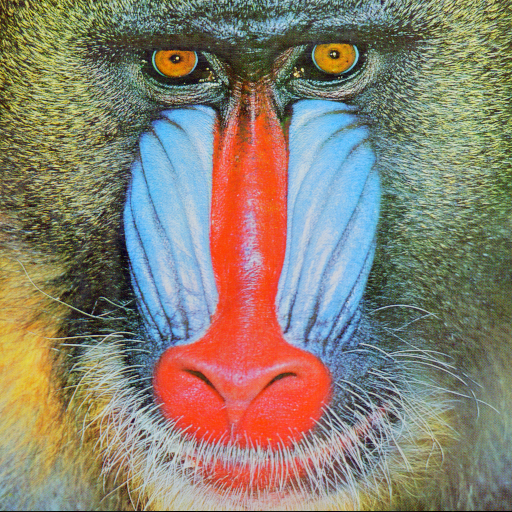
\includegraphics[width=0.4\hsize]{../input/baboon.png}
  
\includegraphics[width=0.4\hsize]{../output/baboon_1.png}
  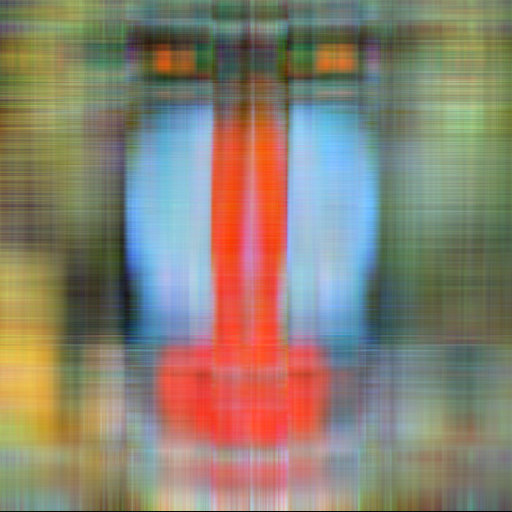
\includegraphics[width=0.4\hsize]{../output/baboon_5.png}
  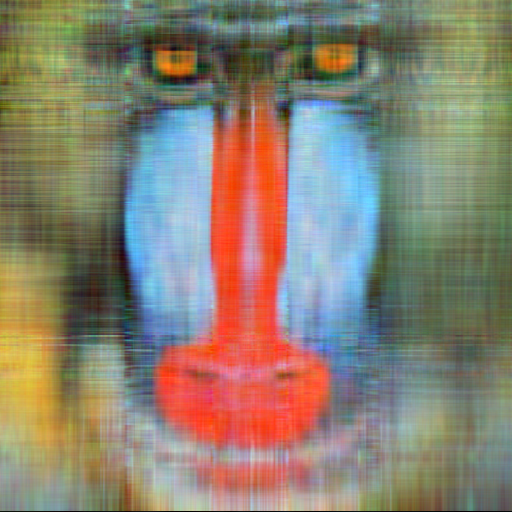
\includegraphics[width=0.4\hsize]{../output/baboon_10.png}
  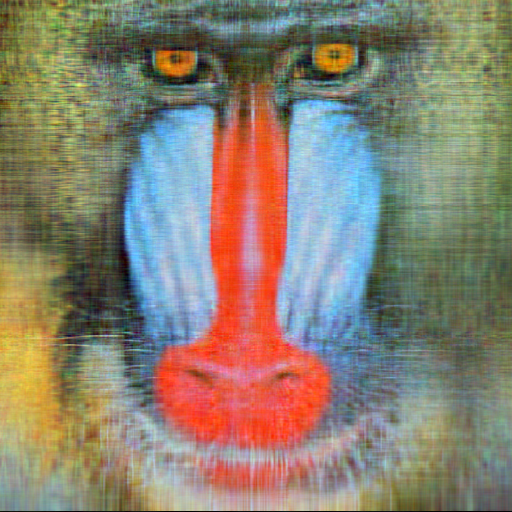
\includegraphics[width=0.4\hsize]{../output/baboon_20.png}
  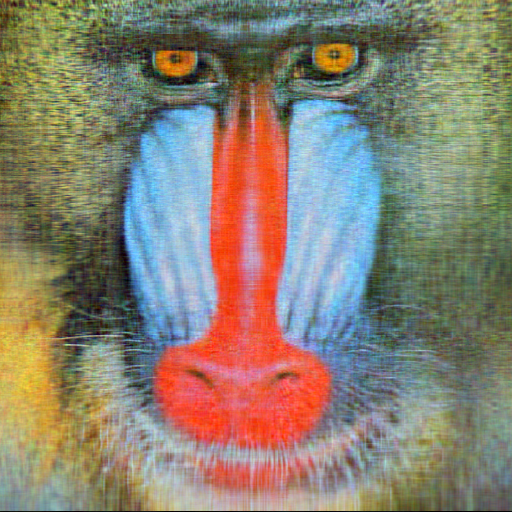
\includegraphics[width=0.4\hsize]{../output/baboon_30.png}
  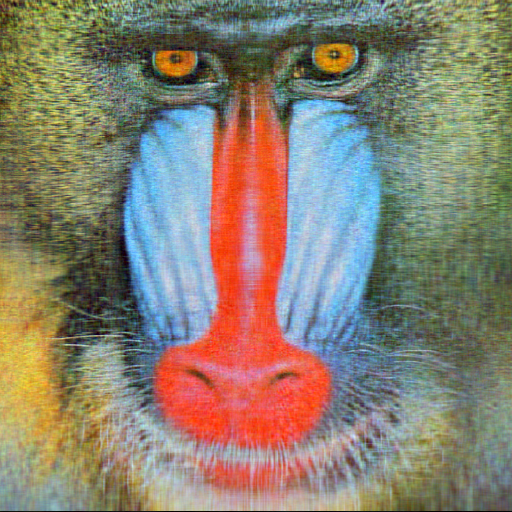
\includegraphics[width=0.4\hsize]{../output/baboon_40.png}
  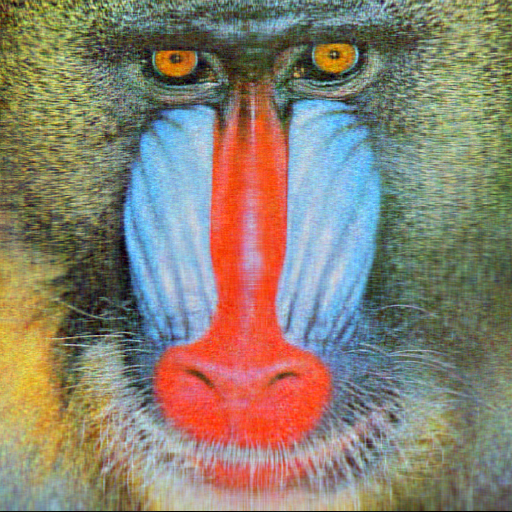
\includegraphics[width=0.4\hsize]{../output/baboon_50.png}
  \caption{Baboon images manipulated in experiments. a) Input. b) Compressed with 1 component. c) Compressed with 5 components. d) Compressed with 10 components e) Compressed with 20 components f) Compressed with 30 components g) Compressed with 40 components h) Compressed with 50 components}
  \label{fig:effect-baboon}
\end{figure}

\begin{figure}[h]
  \centering
  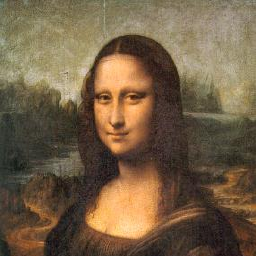
\includegraphics[width=0.4\hsize]{../input/monalisa.png}
  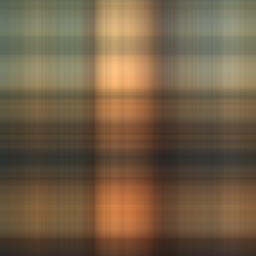
\includegraphics[width=0.4\hsize]{../output/monalisa_1.png}
  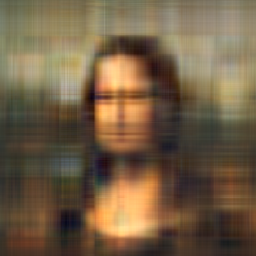
\includegraphics[width=0.4\hsize]{../output/monalisa_5.png}
  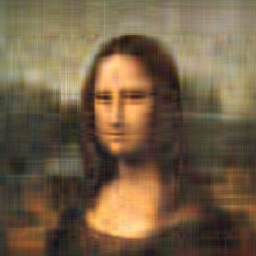
\includegraphics[width=0.4\hsize]{../output/monalisa_10.png}
  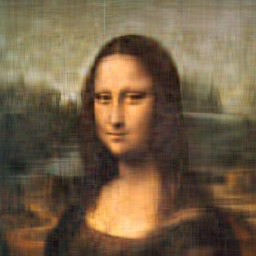
\includegraphics[width=0.4\hsize]{../output/monalisa_20.png}
  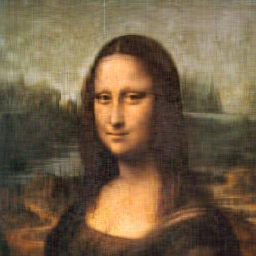
\includegraphics[width=0.4\hsize]{../output/monalisa_30.png}
  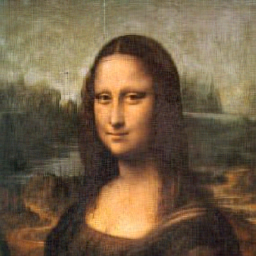
\includegraphics[width=0.4\hsize]{../output/monalisa_40.png}
  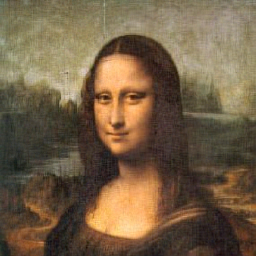
\includegraphics[width=0.4\hsize]{../output/monalisa_50.png}
  \caption{Monalisa images manipulated in experiments. a) Input. b) Compressed with 1 component. c) Compressed with 5 components. d) Compressed with 10 components e) Compressed with 20 components f) Compressed with 30 components g) Compressed with 40 components h) Compressed with 50 components}
  \label{fig:effect-monalisa}
\end{figure}

\begin{figure}[h]
  \centering
  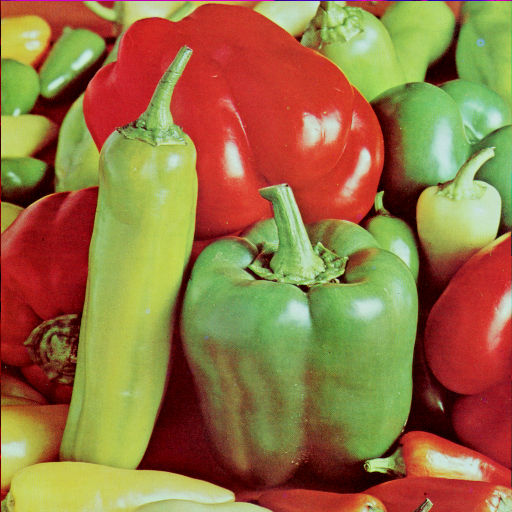
\includegraphics[width=0.4\hsize]{../input/peppers.png}
  
\includegraphics[width=0.4\hsize]{../output/peppers_1.png}
  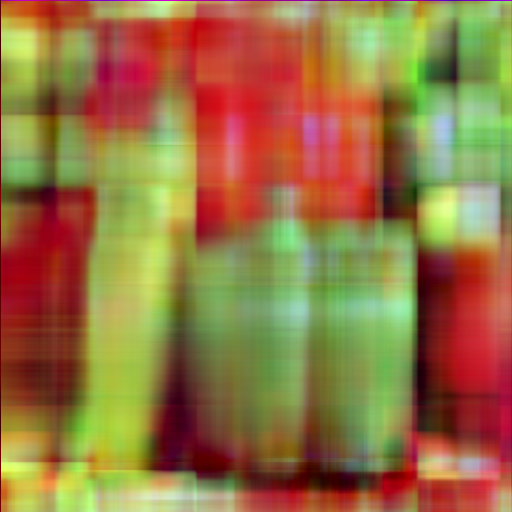
\includegraphics[width=0.4\hsize]{../output/peppers_5.png}
  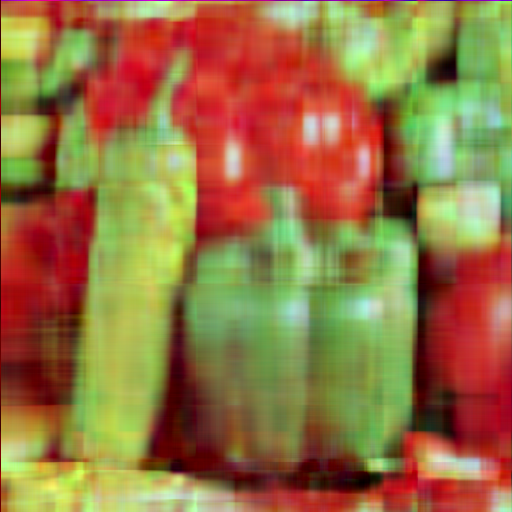
\includegraphics[width=0.4\hsize]{../output/peppers_10.png}
  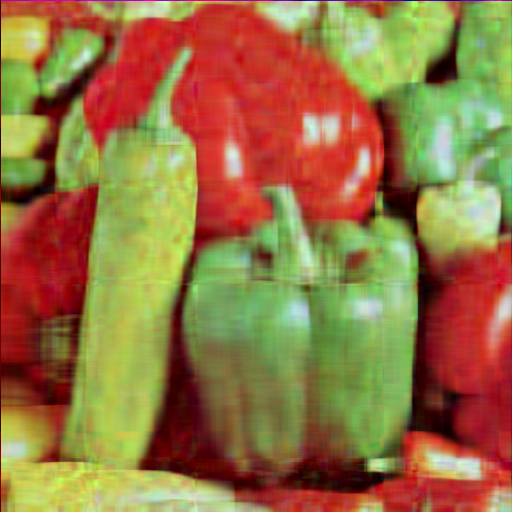
\includegraphics[width=0.4\hsize]{../output/peppers_20.png}
  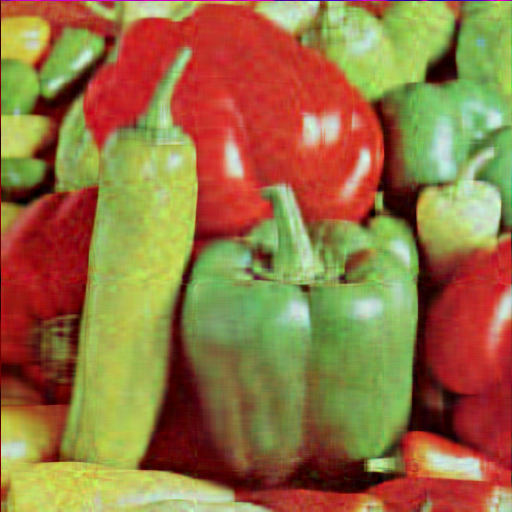
\includegraphics[width=0.4\hsize]{../output/peppers_30.png}
  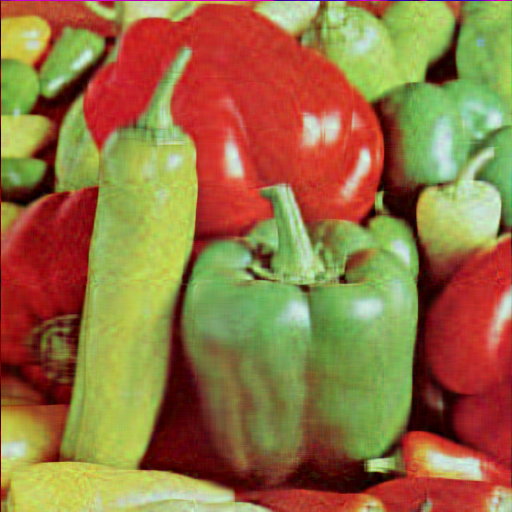
\includegraphics[width=0.4\hsize]{../output/peppers_40.png}
  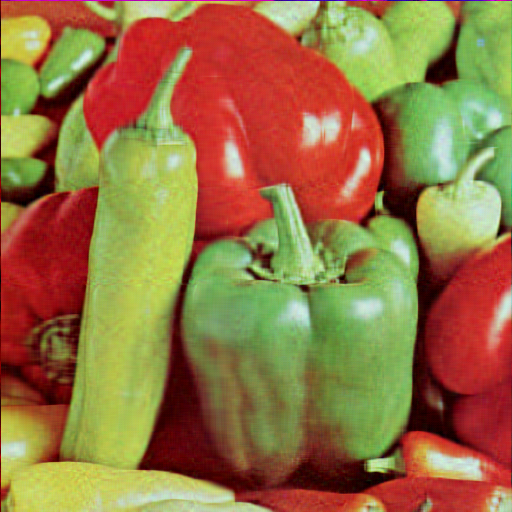
\includegraphics[width=0.4\hsize]{../output/peppers_50.png}
  \caption{Peppers images manipulated in experiments. a) Input. b) Compressed with 1 component. c) Compressed with 5 components. d) Compressed with 10 components e) Compressed with 20 components f) Compressed with 30 components g) Compressed with 40 components h) Compressed with 50 components}
  \label{fig:effect-peppers}
\end{figure}

\begin{figure}[h]
  \centering
  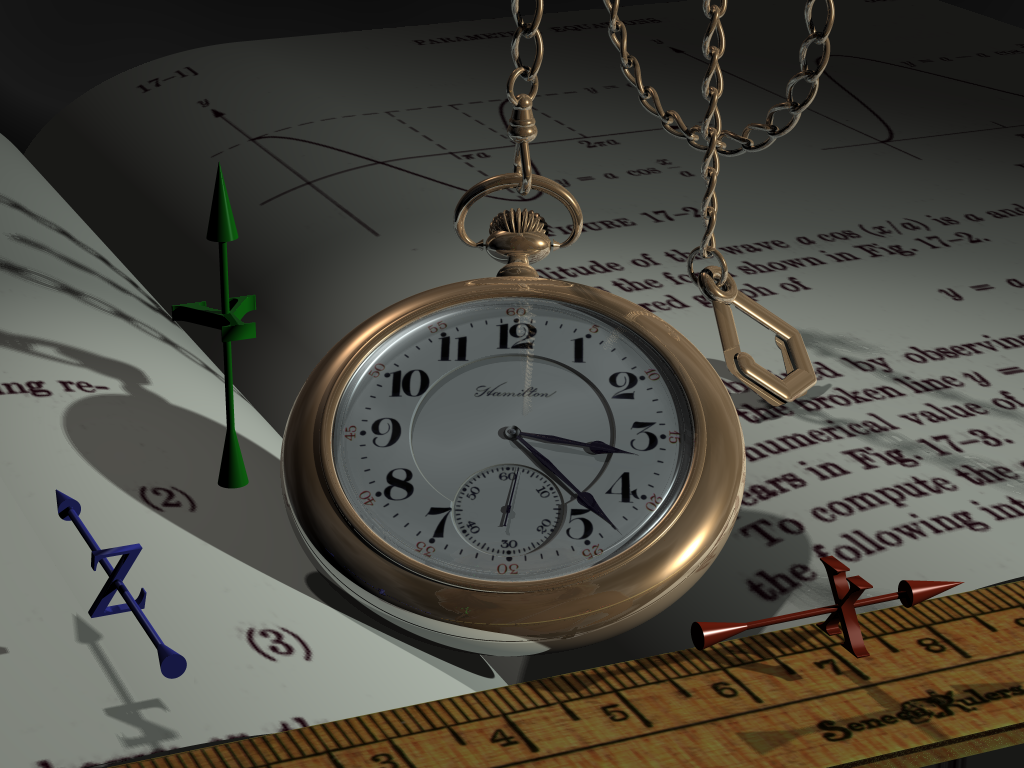
\includegraphics[width=0.4\hsize]{../input/watch.png}
  
\includegraphics[width=0.4\hsize]{../output/watch_1.png}
  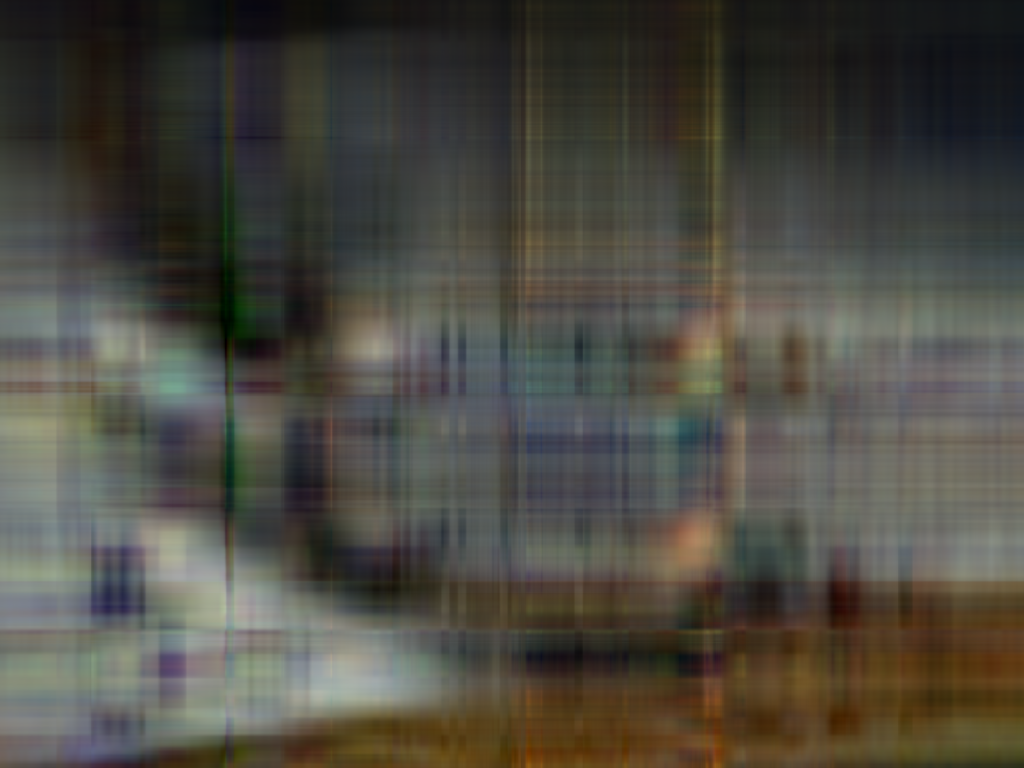
\includegraphics[width=0.4\hsize]{../output/watch_5.png}
  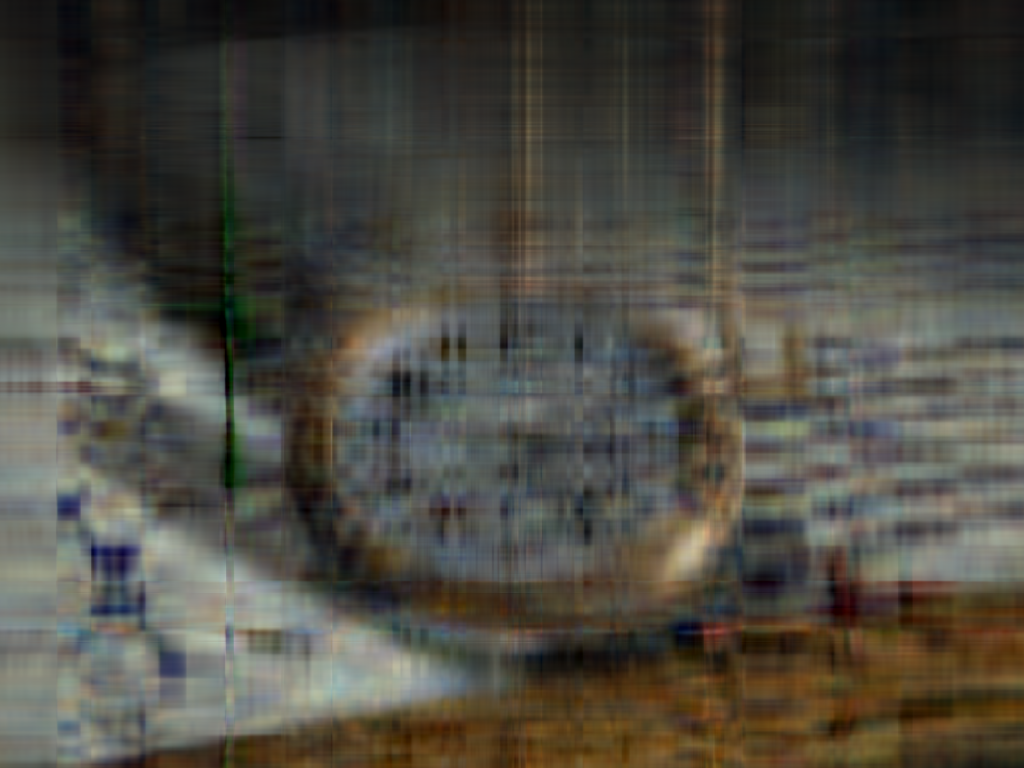
\includegraphics[width=0.4\hsize]{../output/watch_10.png}
  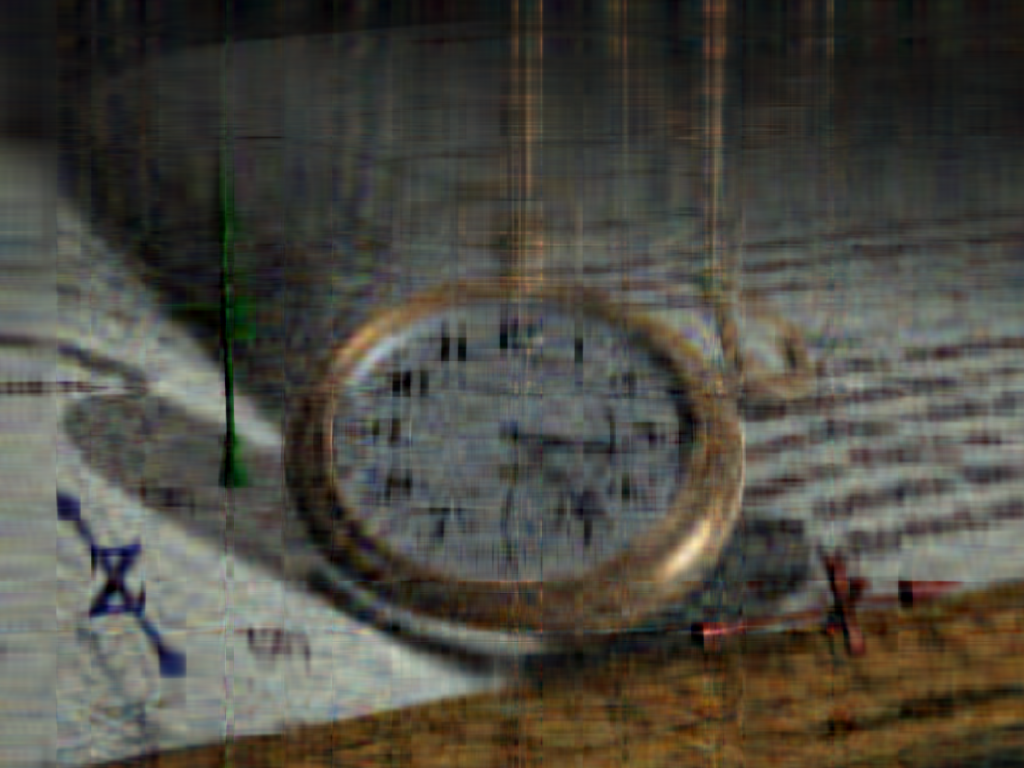
\includegraphics[width=0.4\hsize]{../output/watch_20.png}
  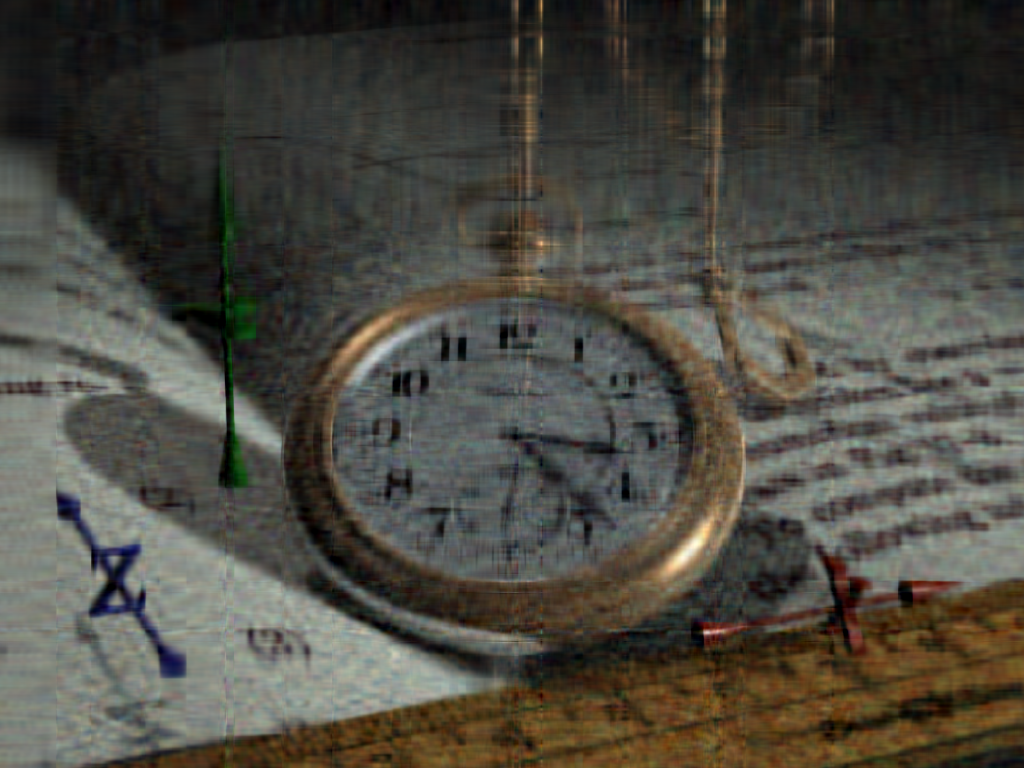
\includegraphics[width=0.4\hsize]{../output/watch_30.png}
  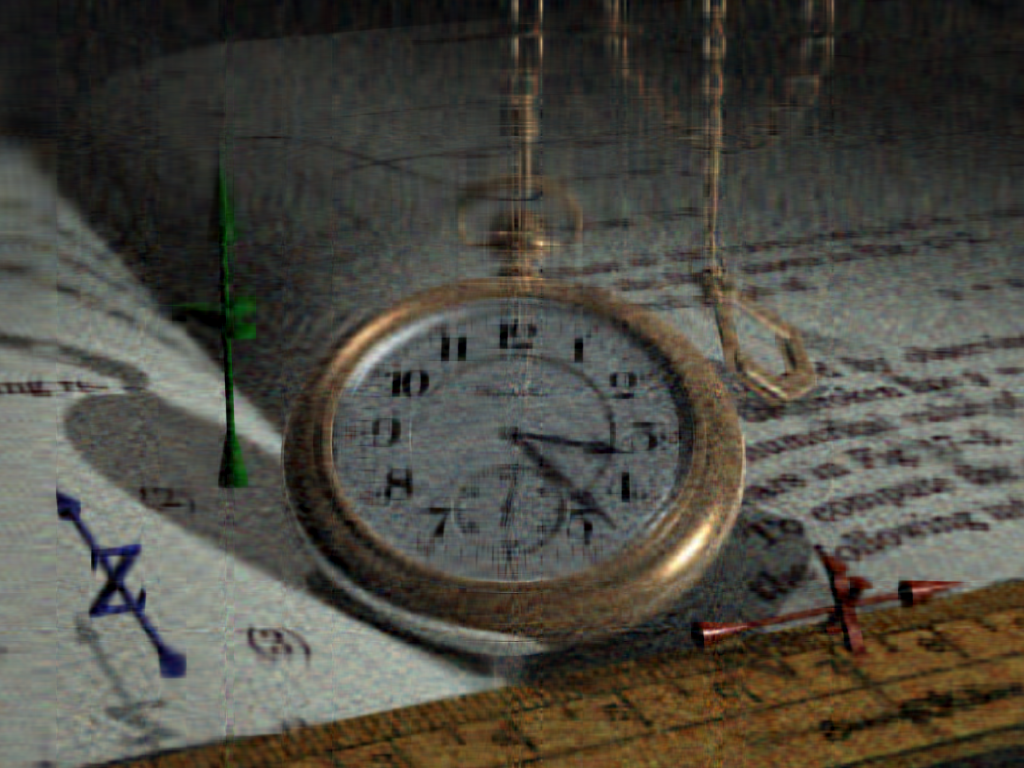
\includegraphics[width=0.4\hsize]{../output/watch_40.png}
  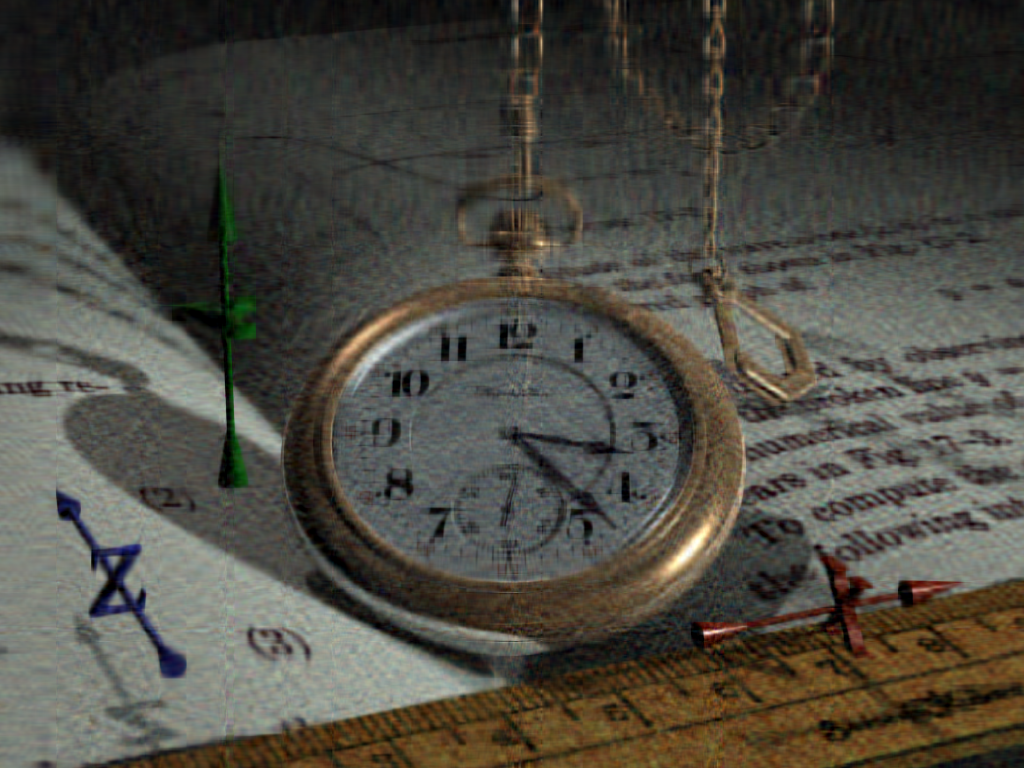
\includegraphics[width=0.4\hsize]{../output/watch_50.png}
  \caption{Watch images manipulated in experiments. a) Input. b) Compressed with 1 component. c) Compressed with 5 components. d) Compressed with 10 components e) Compressed with 20 components f) Compressed with 30 components g) Compressed with 40 components h) Compressed with 50 components}
  \label{fig:effect-watch}
\end{figure}

From the generated images, it is observable the loss of quality created by the process. Even though the greater amount of information is stored in the first component, the image details (high frequency information) is lost from the less significant ones. The higher the dimension and the entropy of the image, the greater is the amount of information loss, because it has more components and more high frequency information. Therefore, the least impacted image is the monalisa one, in which in the last case (50 components), almost half of the components is kept. The most impacted one is the baboon image.  

\subsection{Indicators Results}

In order to analyze the effectiveness of the compression method, the compression rate and RMSE indicators were implemented. The result for all input images are shown in the listings \ref{code:baboon-e}, \ref{code:monalisa-e}, \ref{code:peppers-e} and \ref{code:watch-e}.

\begin{lstlisting}[language=sh, caption={Indicators Results for Baboon Image}, label={code:baboon-e}]
baboon image:
	1 component(s):
		Compression rate: 0.4606994438097151 RMSE:75.38358915100255
	5 component(s):
		Compression rate: 0.605770317267009 RMSE:53.71495530921579
	10 component(s):
		Compression rate: 0.6823673241346407 RMSE:48.29679156656673
	20 component(s):
		Compression rate: 0.7680416577734811 RMSE:43.11258403464472
	30 component(s):
		Compression rate: 0.8153649135582368 RMSE:39.44550826386878
	40 component(s):
		Compression rate: 0.8499196474532009 RMSE:36.36220234788848
	50 component(s):
		Compression rate: 0.8746861228640661 RMSE:33.656196118816396
\end{lstlisting}

For the baboon image, we can see that the quality of the image improves as the number of components increases. In the last case, the compression rate is of 87\%, which shows considerable storage economy, but with a high decrease of quality, shown by the value of the RMSE.

\begin{lstlisting}[language=sh, caption={Indicators Results for Monalisa Image}, label={code:monalisa-e}]
monalisa image:
	1 component(s):
		Compression rate: 0.6481713867848727 RMSE:58.78760860070345
	5 component(s):
		Compression rate: 0.851562288407197 RMSE:26.41430931357357
	10 component(s):
		Compression rate: 0.9292930204844403 RMSE:18.18466943405659
	20 component(s):
		Compression rate: 1.0013361380194463 RMSE:13.001416726457146
	30 component(s):
		Compression rate: 1.0442279740355882 RMSE:10.61092785784305
	40 component(s):
		Compression rate: 1.075094567876714 RMSE:9.060191683551615
	50 component(s):
		Compression rate: 1.0990186607924743 RMSE:7.8451398862882264
\end{lstlisting}

In the case of the monalisa image, we can see an example of how the method does not necessarily work for all images. With more than 20 components, the storage needed for the compressed image is higher than the original input, which shows some failure in the methodology. Also, even though it requires more space, the quality is affected, as some details of the image are lost. With 10 components, the objective is achieved, even though the economy is not as considerable as the quality loss. 

\begin{lstlisting}[language=sh, caption={Indicators Results for Peppers Image}, label={code:peppers-e}]
peppers image:
	1 component(s):
		Compression rate: 0.4759099320834006 RMSE:89.7798662152033
	5 component(s):
		Compression rate: 0.6391102350073967 RMSE:51.023487322642914
	10 component(s):
		Compression rate: 0.7124208119179803 RMSE:37.19033543015182
	20 component(s):
		Compression rate: 0.780881263816731 RMSE:25.239017029794333
	30 component(s):
		Compression rate: 0.815639564992232 RMSE:19.7246540299187
	40 component(s):
		Compression rate: 0.8768201889933902 RMSE:16.34744383844143
	50 component(s):
		Compression rate: 0.8874021111872133 RMSE:14.066020558078767
\end{lstlisting}

For the pappers image, we also have storage economy, with measurable quality loss. The method works better here, as there are less high-frequency information in this case. Still, the RMSE value could be a problem for some applications.

\begin{lstlisting}[language=sh, caption={Indicators Results for Watch Image}, label={code:watch-e}]
watch image:
	1 component(s):
		Compression rate: 0.7172106688702199 RMSE:57.18398114099044
	5 component(s):
		Compression rate: 1.014637274480099 RMSE:40.89070190048771
	10 component(s):
		Compression rate: 1.1777633360877748 RMSE:34.91354161920759
	20 component(s):
		Compression rate: 1.3540734173438003 RMSE:28.577257735650306
	30 component(s):
		Compression rate: 1.4670528623238306 RMSE:24.913312768720537
	40 component(s):
		Compression rate: 1.569728974429601 RMSE:22.31593967903772
	50 component(s):
		Compression rate: 1.6414333998990038 RMSE:20.192015693023528
\end{lstlisting}

For the watch image, the method fails to achieve its objective. The storage required dramatically increases when more components are selected, to the point it surpasses the original image size in the case of only 5, with poor image quality, as shown by the high RMSE.

\section{Conclusion}
The application of the PCA technique to generate compressed versions of images did not succeed for all types of images. For images with high-frequency components, the loss of quality in the output images might be more than expected. The method does not guarantee to decrease the storage requirements for all images.


\bibliography{ref-project} 
\bibliographystyle{ieeetr}

\end{document}
